
\section{Создание экспериментального образца}
//фотография
//характеристики
//процесс сборки
//проверка работы
//перенести подробности из парт2
\subsection{Сборка квадрокоптера}
Первым делом, собирается рама, к ней прикручиваются плата регуляторов и моторы. Делается замер нужной длины проводов моторов и лишняя часть отрезается. Далее все фазы каждого мотора припаиваются на соответствующие площадки регуляторов. Также к регуляторам припаиваются силовые провода с коннектором для подключения аккумулятора. Ставится поверх регулятора полетный контроллер, он подключается к регуляторам через колодку. На передние стойки ставятся пластиковые крепления, куда прикручивается камера, размещается видеопередатчик и производится замер длины проводов, которые необходимо подключить к полетному контроллеру (рис. \ref{fig:quad1}).
% ~\ref{fig:quad1}
\begin{figure}[H]
	\centering
	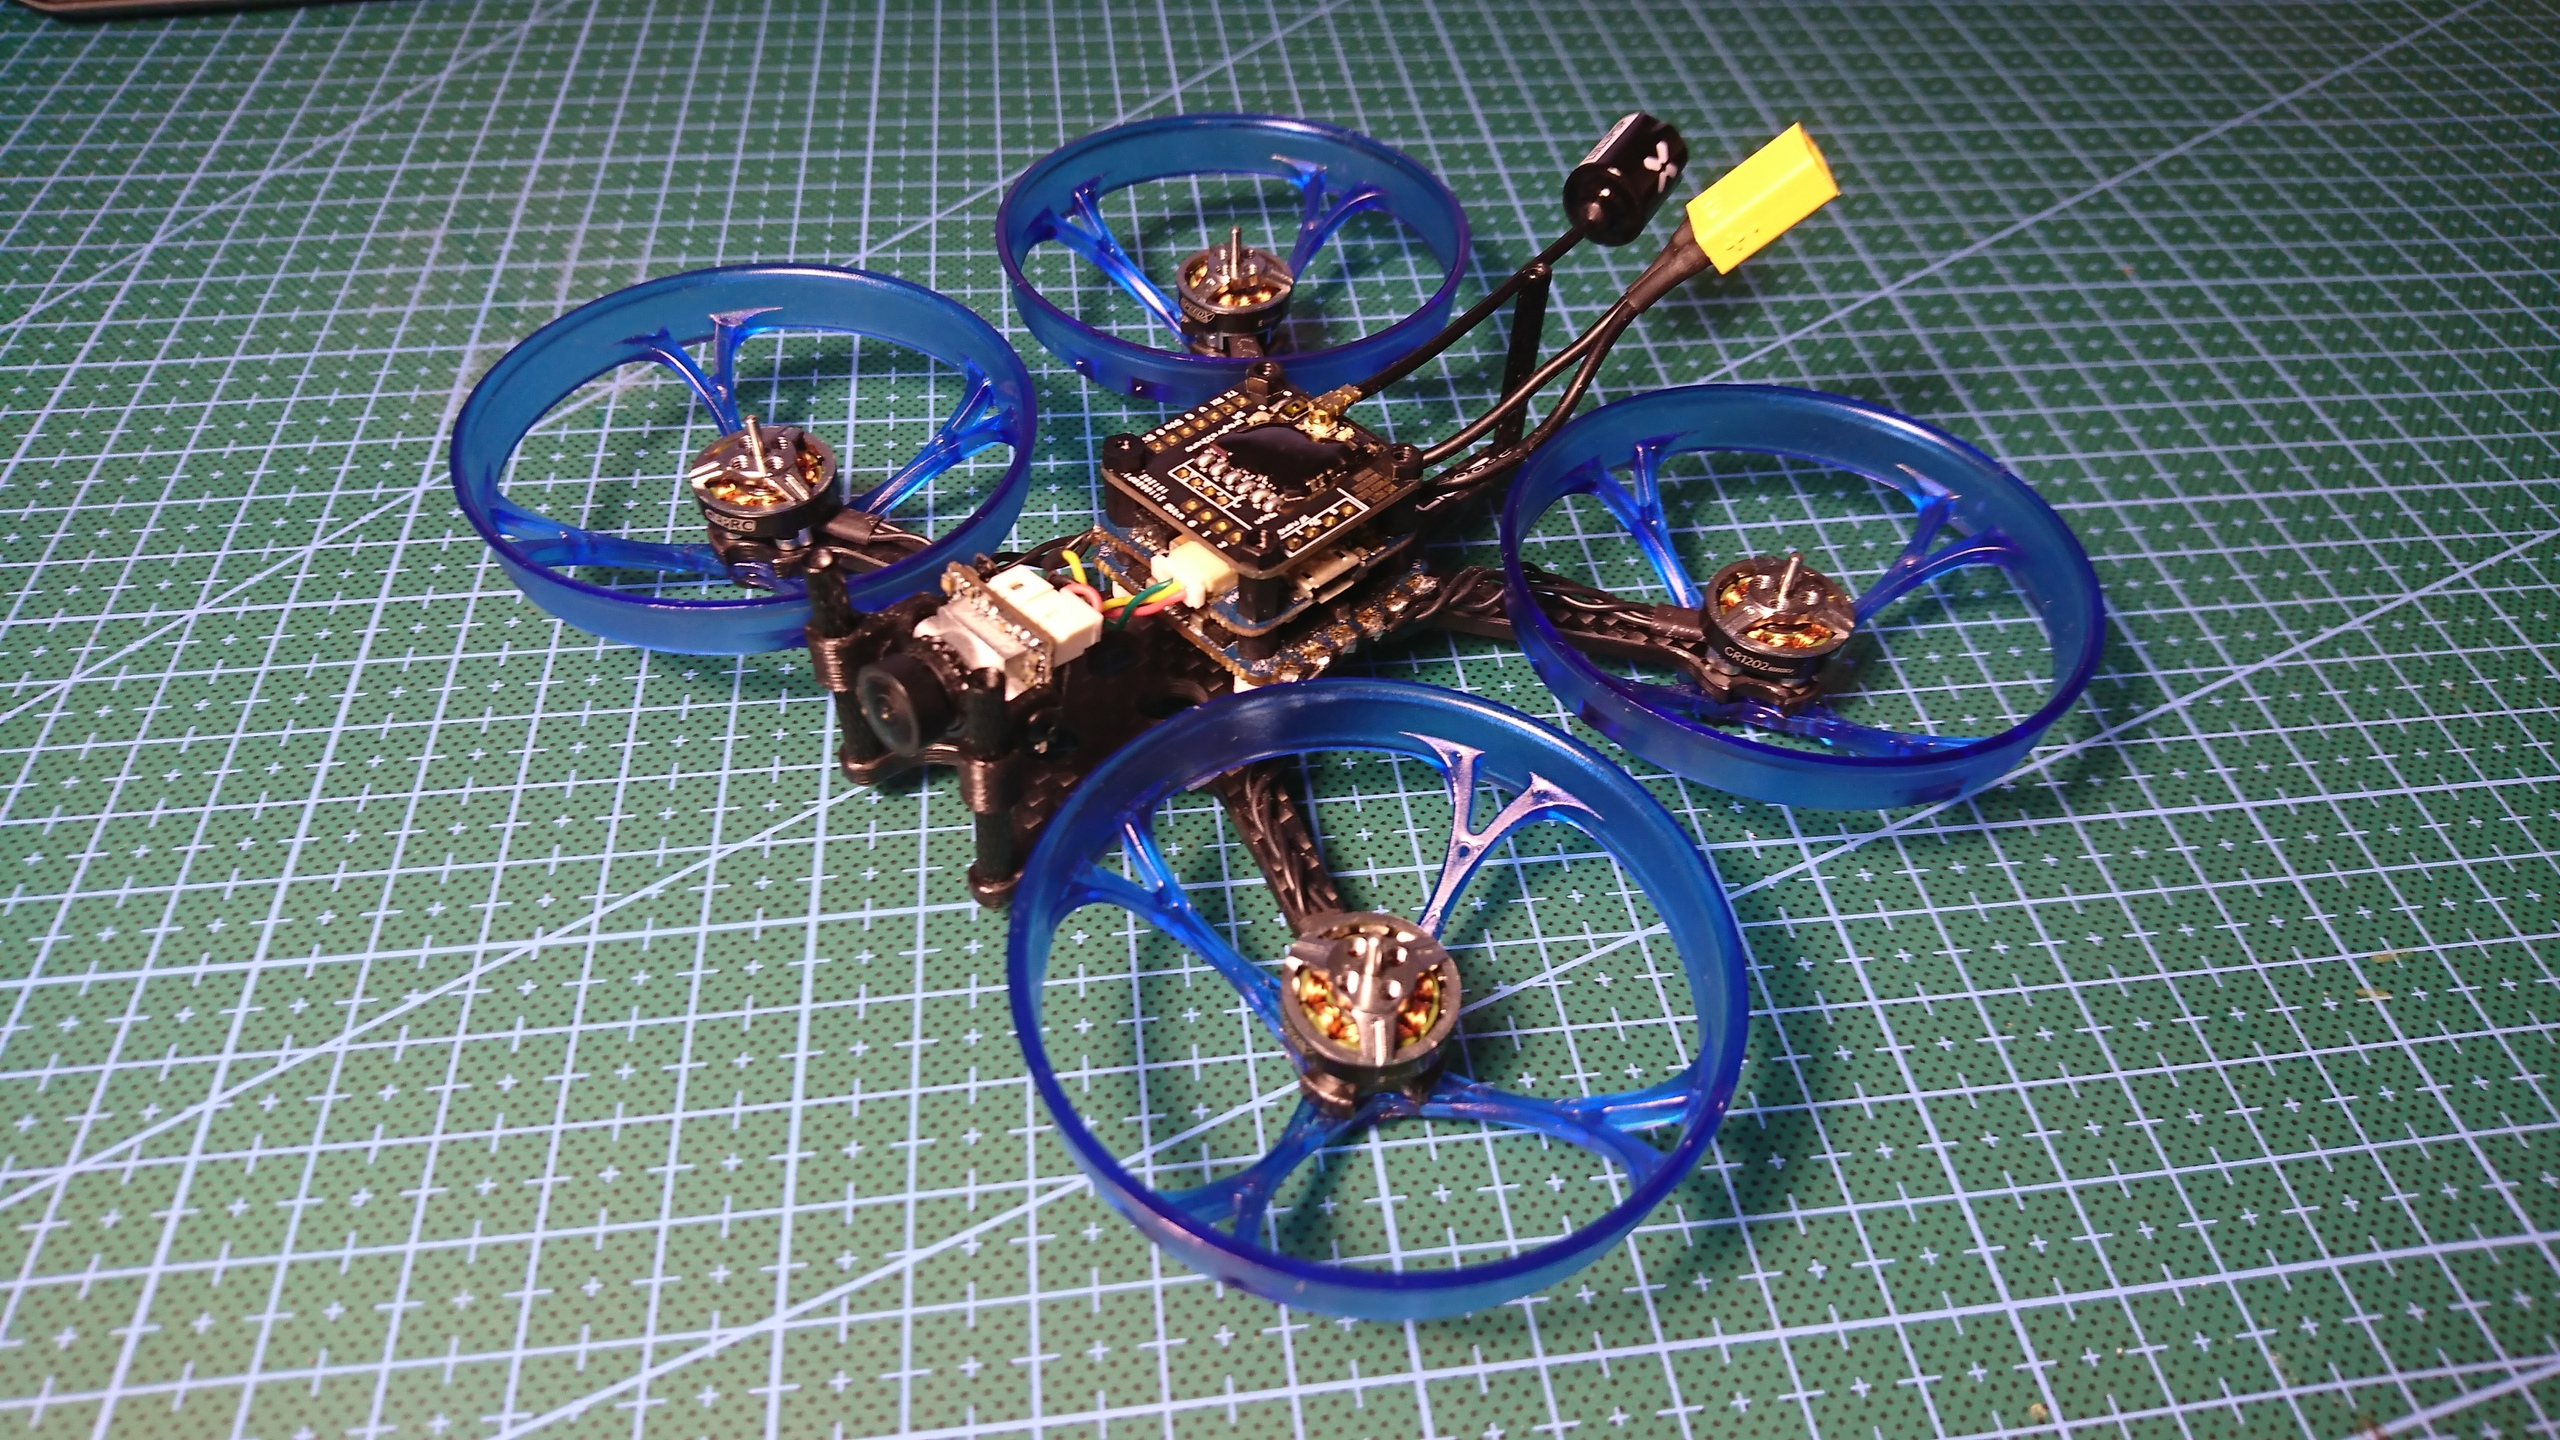
\includegraphics[width=0.5\linewidth]{pics/quad1}
	\caption{Установка компонентов на раму
	}
	\label{fig:quad1}
\end{figure}
После монтажа приемника прикручивается верхняя пластина рамы и на этом сборка завершается (рис. \ref{fig:quad2}).
% ~\ref{fig:quad2}
\begin{figure}[H]
	\centering
	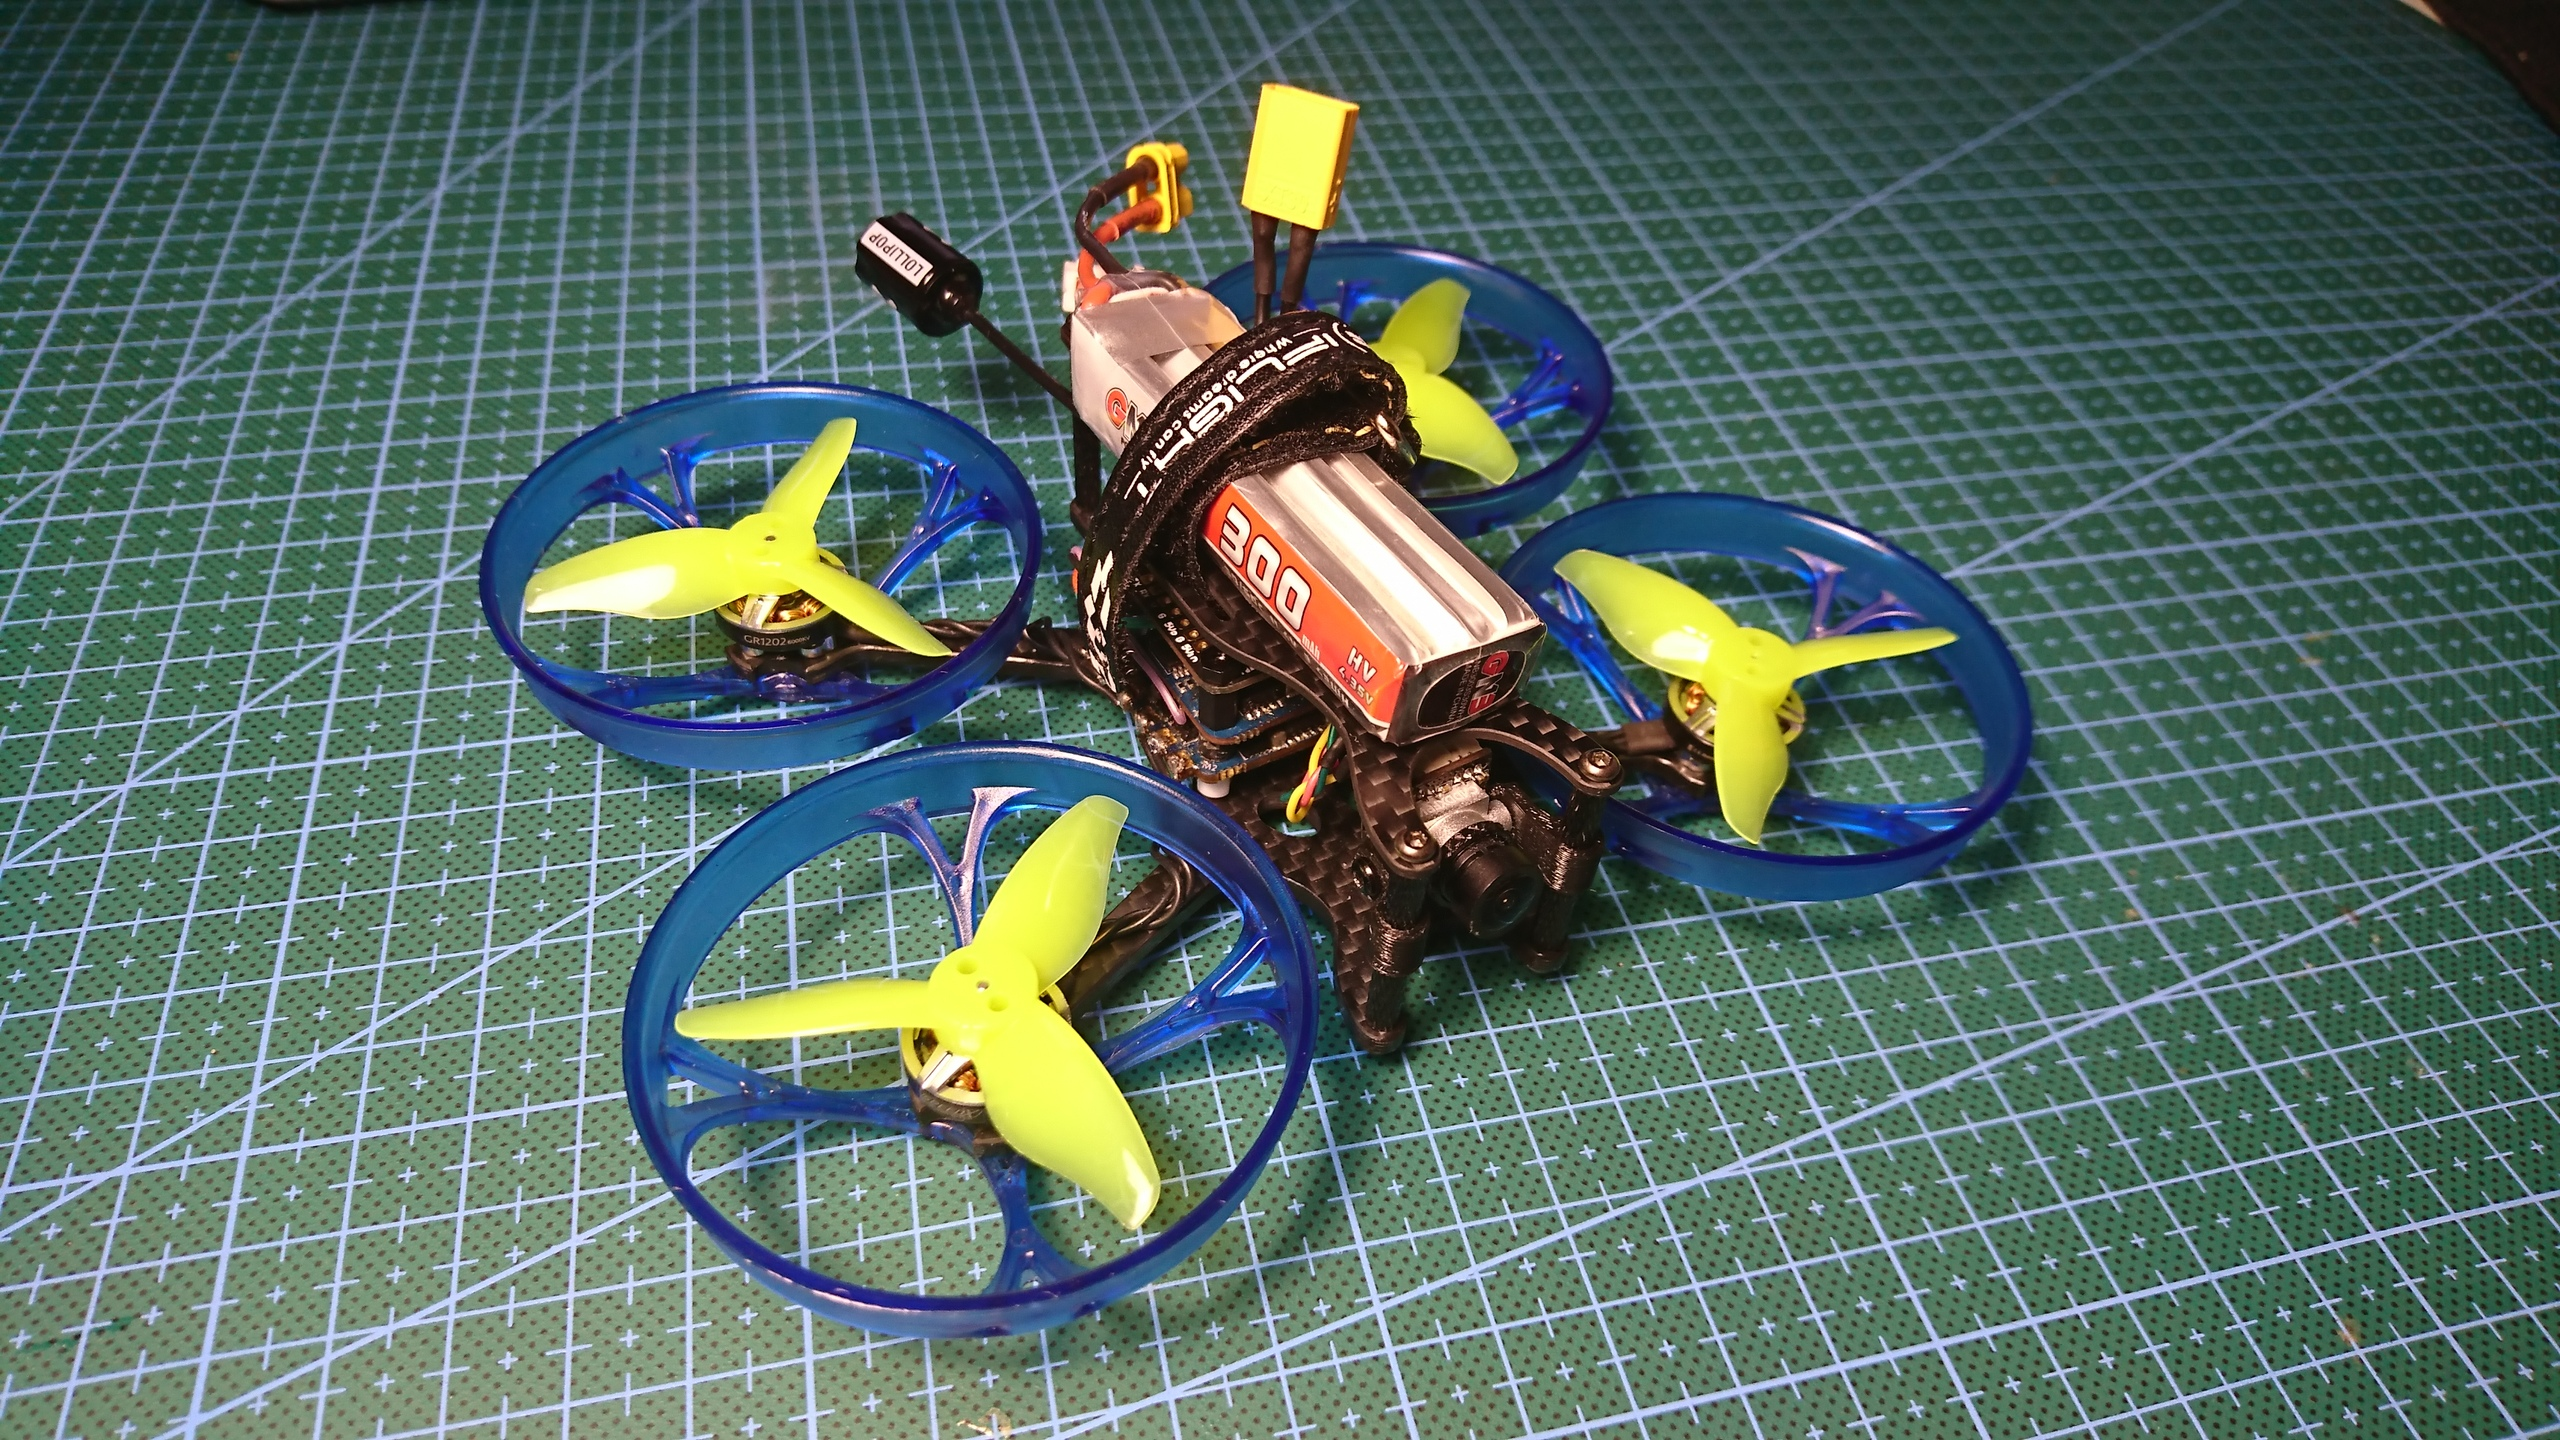
\includegraphics[width=0.5\linewidth]{pics/quad2}
	\caption{Экспериментальный образец квадрокоптера
	}
	\label{fig:quad2}
\end{figure}

\subsection{Сборка наземной станции}

\subsection{Обновление и настройка параметров прошивки}

\subsection{Проверка работы экспериментального образца}
% ~\ref{fig:map}
\begin{figure}[H]
	\centering
	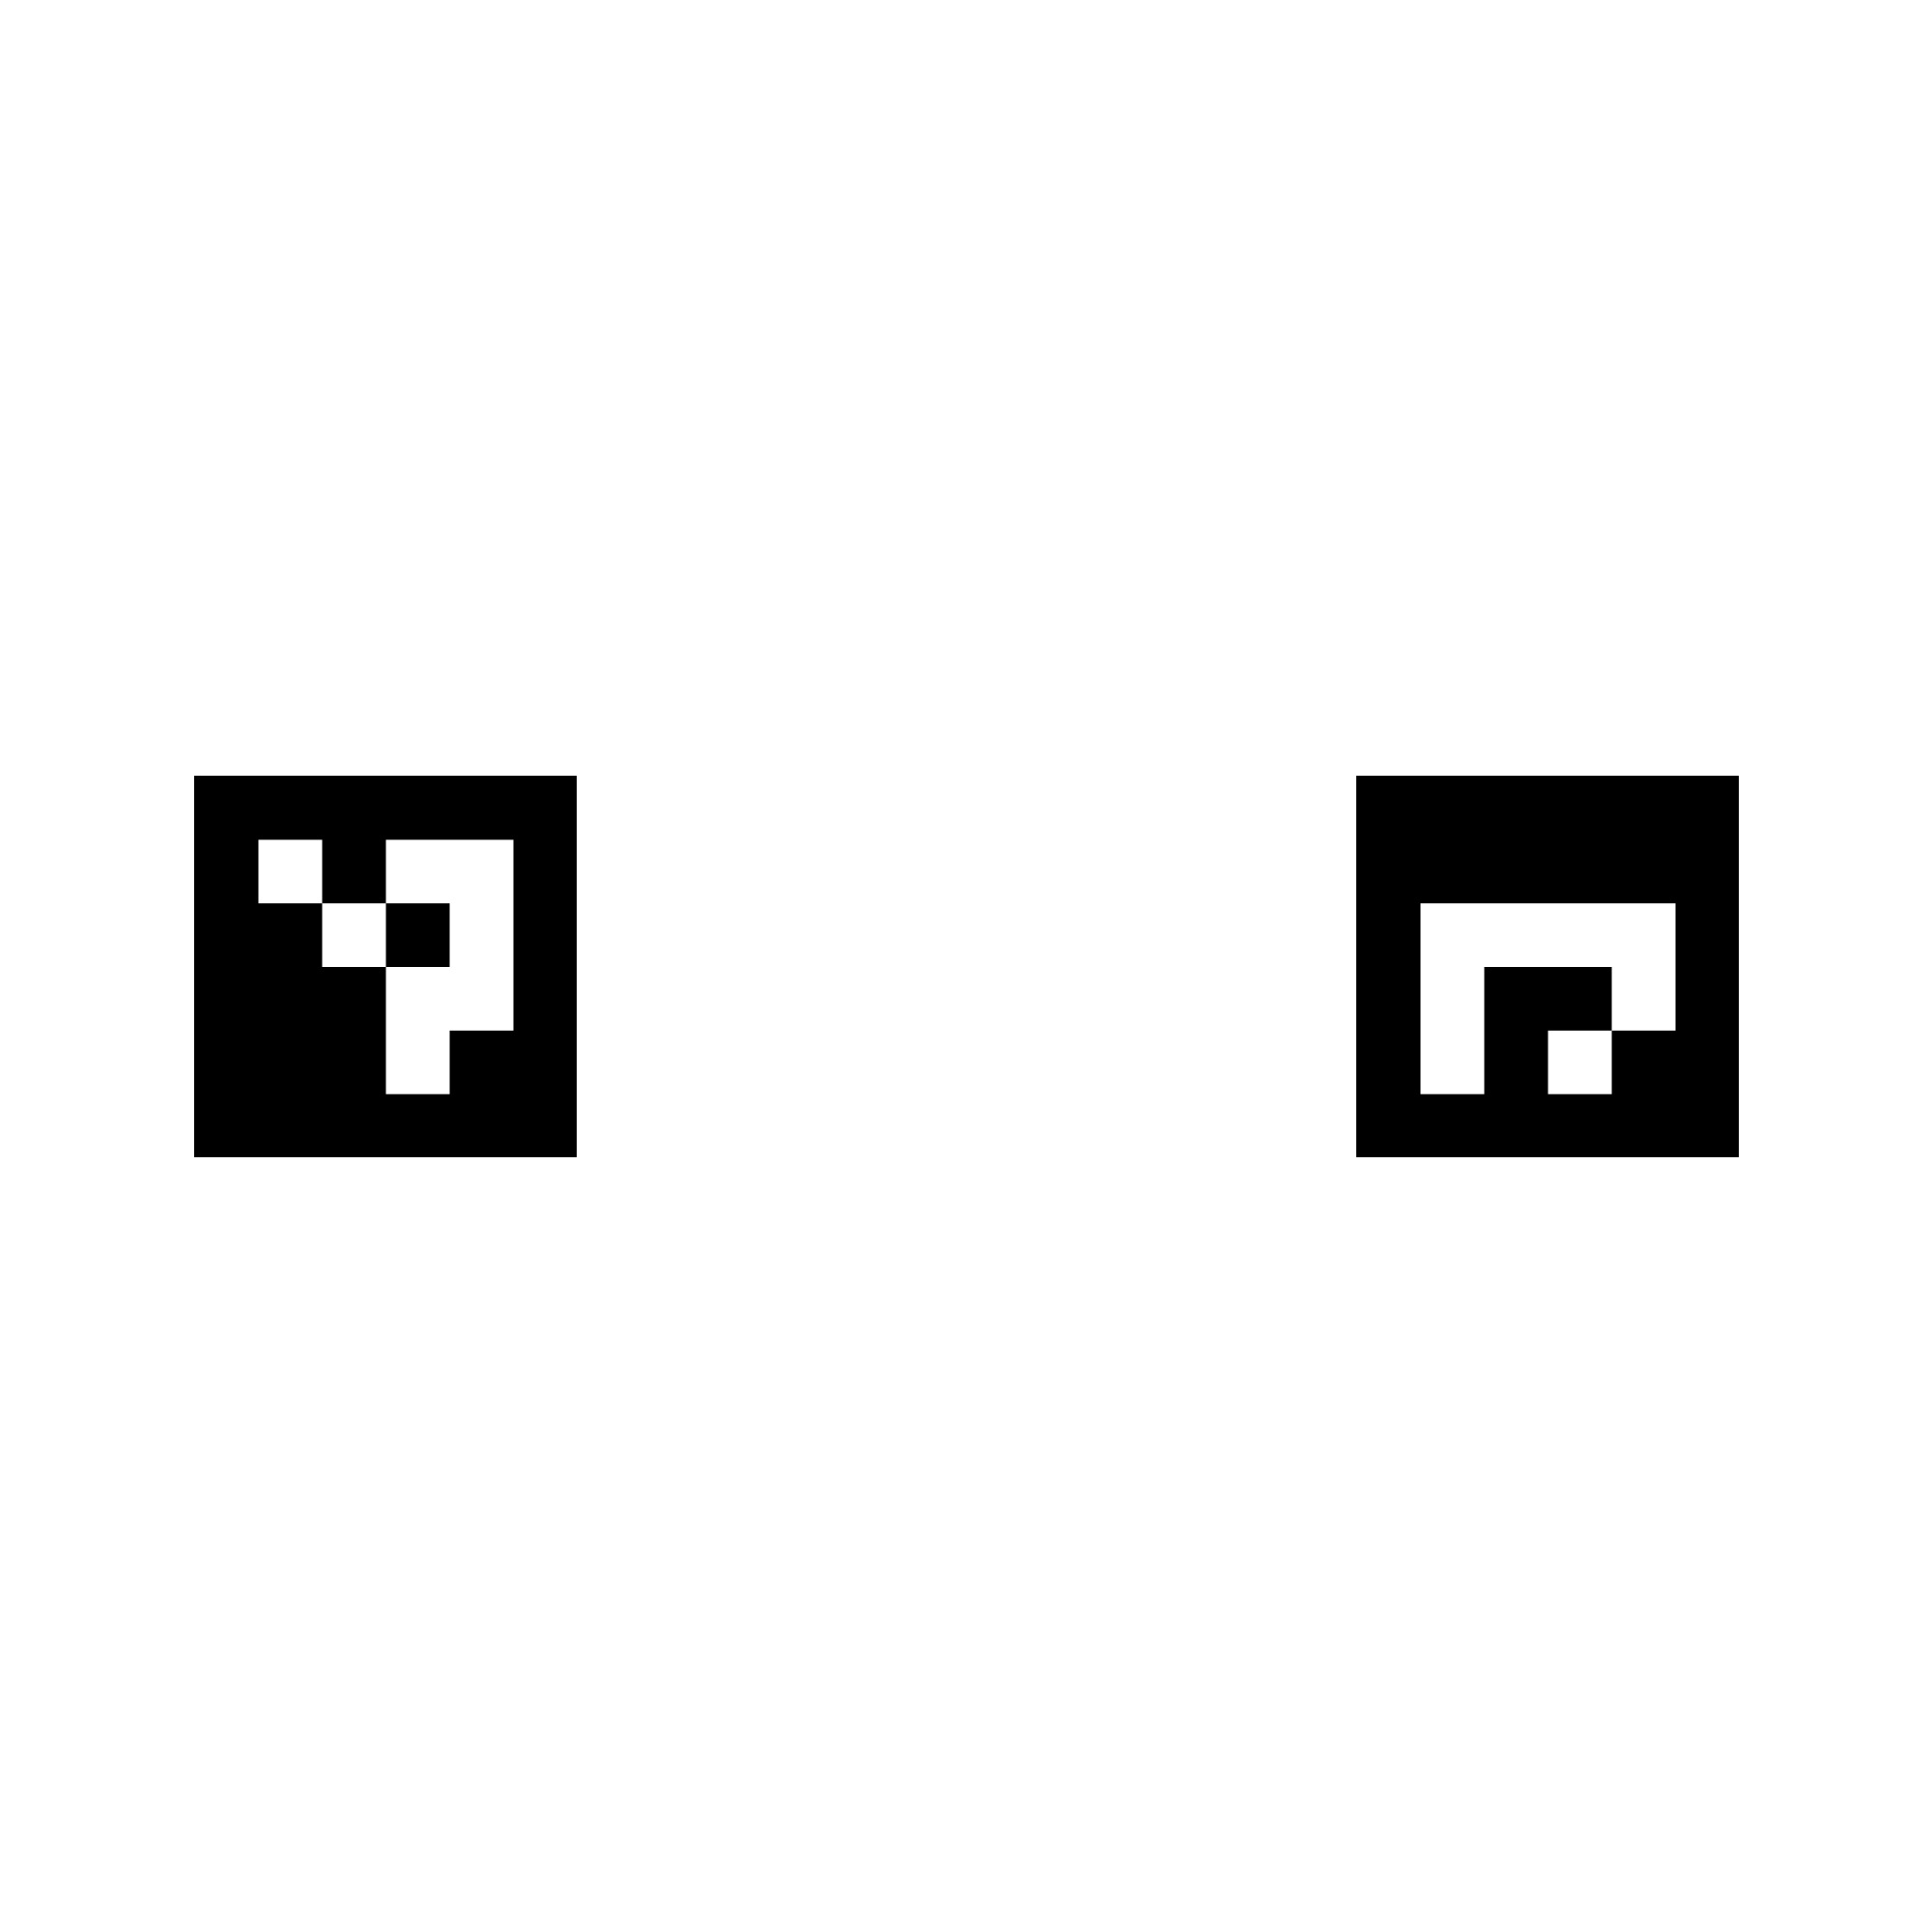
\includegraphics[width=0.5\linewidth]{pics/map}
	\caption{Карта маркеров
	}
	\label{fig:map}
\end{figure}

% ~\ref{fig:aruco_detect}
\begin{figure}[H]
	\centering
	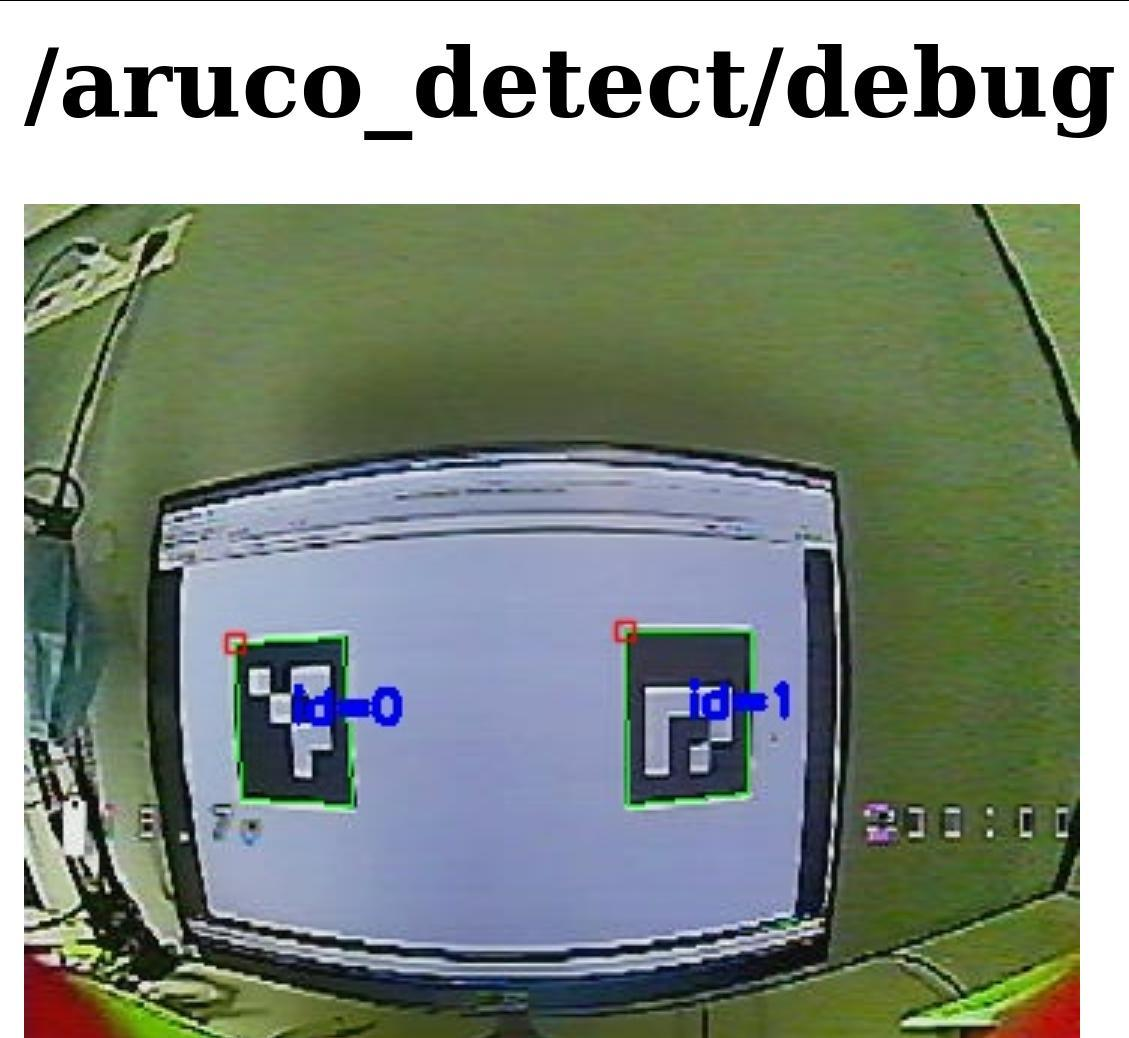
\includegraphics[width=0.5\linewidth]{pics/aruco_detect}
	\caption{Инициализация aruco маркеров
	}
	\label{fig:aruco_detect}
\end{figure}

% ~\ref{fig:time}
\begin{figure}[H]
	\centering
	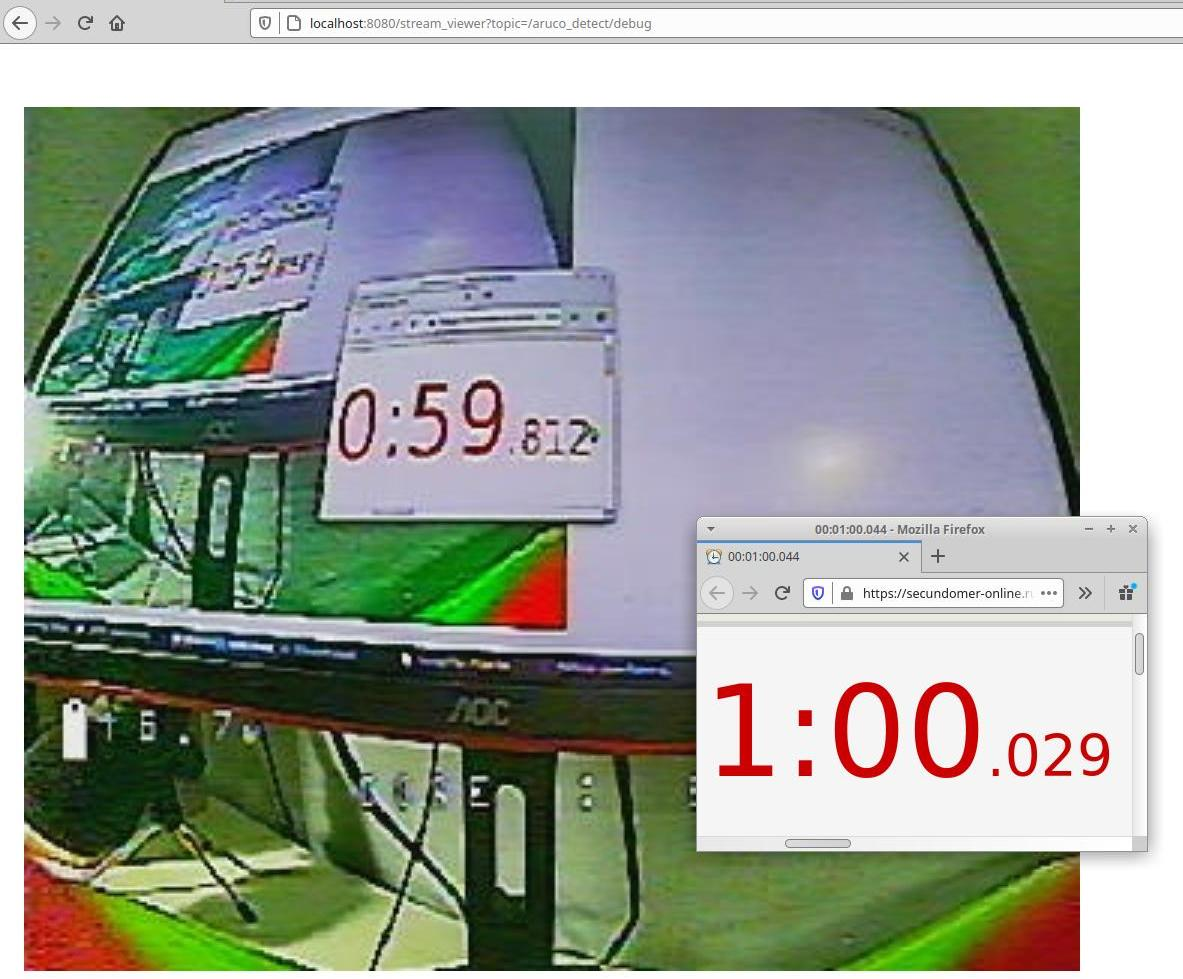
\includegraphics[width=0.5\linewidth]{pics/time}
	\caption{Время задержки% 0.2с
	}
	\label{fig:time}
\end{figure}
